\setcounter{chapter}{3}
\chapter{Resultados}
\section{Introducción}
Los resultados del trabajo de laboratorio reflejan el esquema mismo propuesto en la sección de metodología. Se entrenaron dos aprendices distintos. El primero fue un modelo de predicción ARIMA utilizando como datos la serie de tiempo TRM con información sobre las cotizaciones diarias de la tasa de cambio de los años 2010 a finales del 2017. El segundo modelo fue un aprendiz de regresión multivariable utilizando las series de tiempo TRM como variable dependiente y diferentes regresores de los rubros de exportación. Las salidas de ambos modelos en forma de valores pronosticados fueron utilizados para un tercer aprendiz entrenado utilizando metodologías de modelos ensamblados. Los resultados de cada paso fueron registrados para evaluar el comportamiento y nivel de precisión de cada aprendiz.

\section{Modelo ARIMA}
Para el aprendiz de modelo ARIMA se utilizó la serie de tiempo de la TRM de Colombia con 2,922 puntos de datos abarcando las cotizaciones de la tasa de cambio desde el comienzo del año 2010 hasta el final del año 2017.

\subsection{Validación de los Datos de Entrada}
La evaluación de la serie de tiempo previo al uso concluye que la misma estaba completa y sin datos que ameriten imputación. Para validar dicha aseveración se reviso primero el rango de datos y luego la visualización de la serie descompuesta en tendencia secular, variación estacionaria y error aleatorio.

La determinación del rango abarcó valores con un mínimo de 1,557 y un máximo de 3,414:

\begin{table}[h!]
  \begin{center}
    \caption{Rango de Valores Serie de Tiempo TRM}
    \label{tab:table1}
    \begin{tabular}{c|c|c|c|c|c}
      \textbf{Min.} & \textbf{1st Qu.} & \textbf{Median} & \textbf{Mean} & \textbf{3rd Qu.} & \textbf{Max.}\\
      \hline
      1557 & 1828 & 1933 & 2259 & 2906 & 3414\\
    \end{tabular}
  \end{center}
\end{table}

El análisis visual de la serie de tiempo determinó que a lo largo de su extensión no se vislumbraron valores extremos, nulos u otro tipo de anormalidad que afectara el entrenamiento.

\begin{figure}[h!]
    \centering
    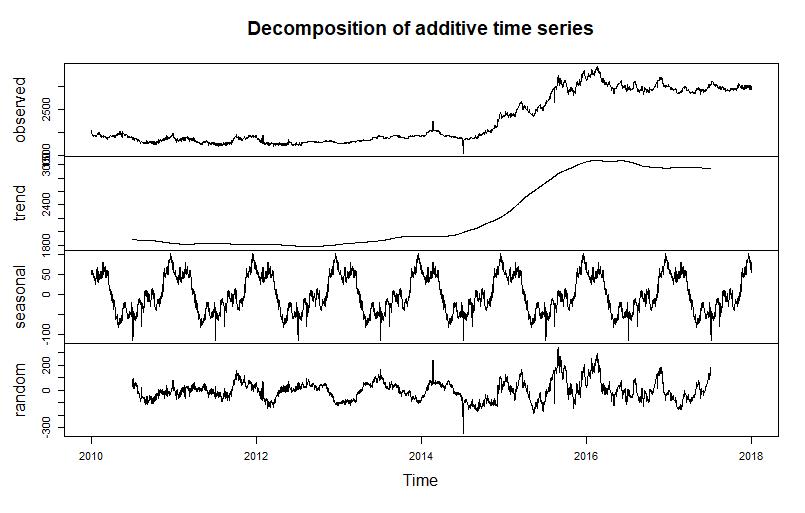
\includegraphics[width = 6 in]{decomposicionTRM.png}
    \caption{Descomposición de la Serie de Tiempo TRM 2010-2017}
\end{figure}

La serie de tiempo TRM tiene una marcada variación estacional por lo que no es estacionaria. El análisis visual determina que la TRM responde a patrones por temporada de fluctuaciones previsibles, adicionalmente sumado a una tendencia alcista que alcanzó un plató en el año 2017. La idea de una estacionalidad marcado se verifica con el análisis de autocorrelación y autocorrelación parcial efectuado en la serie.

\begin{figure}[H]
    \centering
    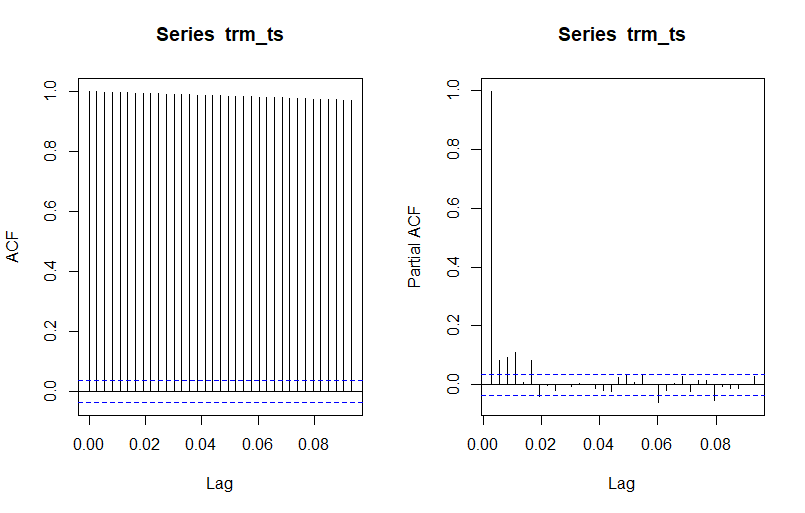
\includegraphics[width = 6 in]{autocorrelacionTRM.png}
    \caption{Análisis de Autocorrelación y Correlación Parcial de la Serie de Tiempo TRM 2010-2017}
\end{figure}

El primer gráfico demuestra que la serie de tiempo TRM tiene una autocorrelación marcada donde cada valor de cotización se da en función del anterior. La autocorrelación parcial demuestra que fuera del primer retraso la serie no presenta autocorrelación en períodos superiores.

\subsection{Entrenamiento de Datos}
Posteriormente al análisis EDA la serie de tiempo se entrenó con la metodología ARIMA utilizando la función \emph{auto.Arima()} de la biblioteca \emph{forecast} creada por el Dr. Hyndmann \cite{hyndman}. Los resultados resumidos del entrenamiento fueron los siguientes.

\begin{lstlisting}[language=R]
Series: trm_ts
ARIMA(3,1,2)

Coefficients:
          ar1     ar2      ar3     ma1      ma2
      -0.3578  0.2932  -0.1187  0.2176  -0.4763
s.e.   0.0852  0.0770   0.0226  0.0848   0.0760

sigma^2 estimated as 654:  log likelihood=-13610.88
AIC=27233.77   AICc=27233.8   BIC=27269.65

Training set error measures:
                    ME     RMSE      MAE        MPE      MAPE       MASE         ACF1
Training set 0.5077876 25.54737 14.28794 0.01199701 0.6205936 0.06057789 0.0001886243
\end{lstlisting}

El modelo final entrenado es del tipo ARIMA(3,1,2). El error promedio del modelo entrenado se ubica en 0.5078 y el error cuadrático en 25.55 (esto último debe entenderse como pesos colombianos). La ecuación del modelo ARIMA se puede escribir como:

\begin{equation}
    \Delta y_t = -0.3578 \Delta y_{t-1} + 0.2932 \Delta y_{t-2} - 0.1187 \Delta y_{t-3} + 0.2176 \epsilon_{t-1} -
    0.4763 \epsilon_{t-2}
\end{equation}

donde $\Delta = y_{t} - y_{t-1}$

\subsection{Validación del Modelo Entrenado}
Para comprender mejor el calce de los valores de predicción se graficó los valores reales del juego de entrenamiento versus los valores esperados del modelo en la tabla 4.3.

\begin{figure}[H]
    \centering
    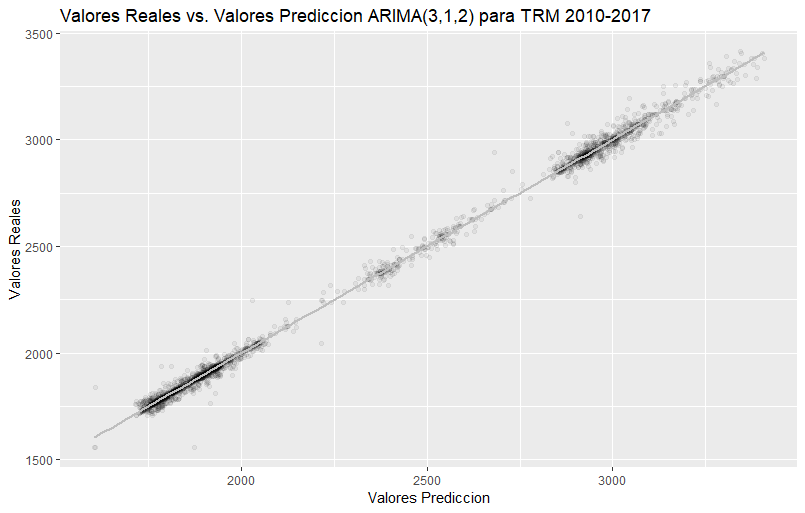
\includegraphics[width = 5 in]{realVStrainingARIMA.png}
    \caption{Análisis Valores Reales vs. Predicción Entrenamiento ARIMA de la Serie de Tiempo TRM 2010-2017}
\end{figure}

El coeficiente $R^2$ - coeficiente de determinación - del calce de los valores es 0.9976 con un valor de $p-value: < 2.2e-16$.

Dado que la función automática de entrenamiento ARIMA de la biblioteca \emph{forecast} utiliza los 2,922 puntos de datos para entrenar a través del muestreo múltiple con ventanas se procedió a revisar la precisión del modelo con una función de ayuda que determina diez puntos de datos al azar y calcula el error promedio entre valores reales de la TRM y los valores de predicción. Los valores del test se reflejan en la siguiente tabla:

\begin{lstlisting}[language=R]
> print(testMatrix)
   VALOR REAL PREDICCION ERROR %
1      2144.5   2144.517     0.0
2      1833.0   1829.345    -0.2
3      1930.0   1931.454     0.1
4      2031.0   2035.333     0.2
5      2049.0   2044.812    -0.2
6      1753.8   1757.048     0.2
7      2546.0   2533.526    -0.5
8      1817.0   1816.756     0.0
9      1819.2   1815.438    -0.2
10     1927.0   1925.947    -0.1
> print(mean(testMatrix$`ERROR %`))
[1] -0.07
>
\end{lstlisting}

Como procedimiento de evaluación final se visualizó una gráfica con cien valores aleatorios de prueba y su calce.
\begin{figure}[H]
    \centering
    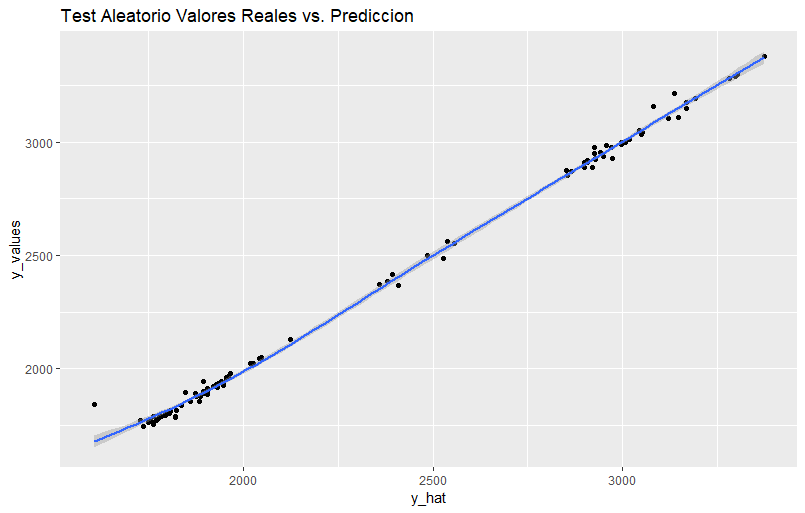
\includegraphics[width = 5 in]{testAleatorioARIMA.png}
    \caption{Test Aleatorio Valores Reales vs. Predicción Entrenamiento ARIMA TRM 2010-2017}
\end{figure}

\section{Modelo Regresión Lineal Multivariable}
Para la evaluación del modelo de regresión lineal multivariable se utilizó once juegos de datos diferentes correspondientes a la variable de predicción TRM y diez series de tiempo representativas de los diez rubros principales de exportación de Colombia:

\begin{itemize}
  \item el petroleo West Texas
  \item el gasoleo (también conocido como gasoil)
  \item el polipropileno
  \item el carbón
  \item el café
  \item el aceite de palma
  \item el guineo (también conocido como banano)
  \item el oro
  \item el ferroníquel
  \item la hulla térmica
\end{itemize}

\subsection{Validación de los Datos de Entrada}
Previo a la utilización de los datos en el entrenamiento, se procedió a validar que las once series de datos estuviesen completas con la misma cantidad de puntos de información, 2,922 en cada caso, sin valores extremos u omitidos.

El primer examen se validó con la estructura de datos para cada serie de tiempo.

\begin{lstlisting}[language=R]

     Date                 trm           palma
 Min.   :2010-01-01   Min.   :1557   Min.   : 483.5
 1st Qu.:2012-01-01   1st Qu.:1828   1st Qu.: 634.4
 Median :2013-12-31   Median :1933   Median : 752.9
 Mean   :2013-12-31   Mean   :2259   Mean   : 779.4
 3rd Qu.:2015-12-31   3rd Qu.:2906   3rd Qu.: 883.5
 Max.   :2017-12-31   Max.   :3414   Max.   :1248.5

  oro            wti              cafe
Min.   :1049   Min.   : 26.19   Min.   :101.5
1st Qu.:1214   1st Qu.: 50.25   1st Qu.:128.1
Median :1286   Median : 82.53   Median :144.8
Mean   :1350   Mean   : 75.29   Mean   :162.0
3rd Qu.:1475   3rd Qu.: 96.08   3rd Qu.:182.4
Max.   :1895   Max.   :113.39   Max.   :304.9


     banana           niquel          gasoil
 Min.   : 782.7   Min.   : 8298   Min.   : 251.1
 1st Qu.: 926.1   1st Qu.:10348   1st Qu.: 470.0
 Median : 955.4   Median :15756   Median : 992.0
 Mean   : 964.2   Mean   :15714   Mean   : 799.8
 3rd Qu.:1004.7   3rd Qu.:19055   3rd Qu.:1054.9
 Max.   :1151.4   Max.   :28412   Max.   :1112.4

      polipropileno       hulla          carbon
 Min.   : 98.3   Min.   :4100   Min.   :39.55
 1st Qu.:100.0   1st Qu.:4450   1st Qu.:52.60
 Median :104.4   Median :7888   Median :60.15
 Mean   :104.0   Mean   :6563   Mean   :60.03
 3rd Qu.:107.0   3rd Qu.:7888   3rd Qu.:67.27
 Max.   :109.1   Max.   :8510   Max.   :81.65
\end{lstlisting}

Todos los datos se ajustaron a las fechas de inicio del año 2010 y finales del 2017, sin la existencia de valores nulos o extremos. Una segunda verificación visual se dió al graficar todas las series de datos en una matriz de valores correspondiente al gráfico 4.5.

\begin{figure}[H]
    \centering
    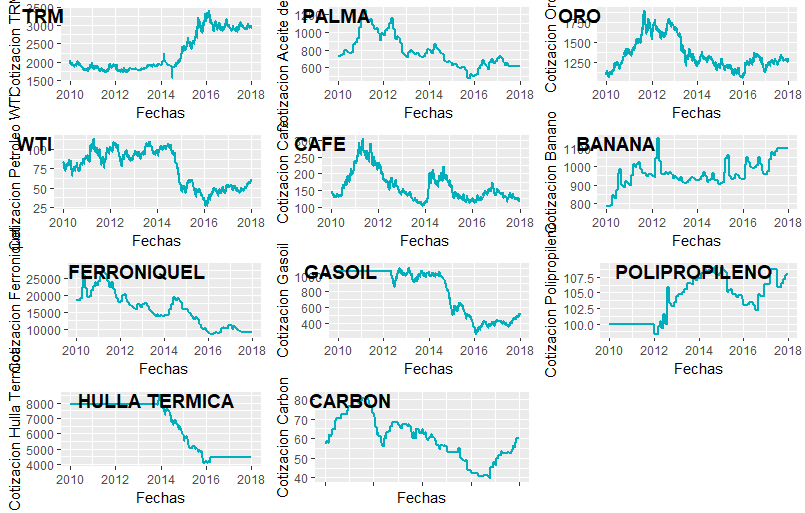
\includegraphics[width = 6 in]{matrizTS.png}
    \caption{Matriz Series de Tiempo 2010-2017 Modelo Regresión Lineal}
\end{figure}

\subsection{Entrenamiento de Datos}
Previo al entrenamiento de los datos se procedió a un pre-análisis EDA para evaluar la correlación de los mismos. El modelo no esta entrenado sino que solamente calculó la regresión multivaraible de los regresores utilizando la serie de tiempo TRM como variable independiente. El correlograma resultante evidencia diferentes niveles de correlación de cada uno de los regresores que varian en su nivel de ajuste. Los coeficientes de determinación más débiles se dieron con los regresores de banana ($R^2 = 0.45$) y polipropileno ($R^2 = 0.36$) mientras que los más fuertes se dieron con la hulla ($R^2 = 0.97$) y carbón ($R^2 = 0.97$).

\begin{figure}[H]
    \centering
    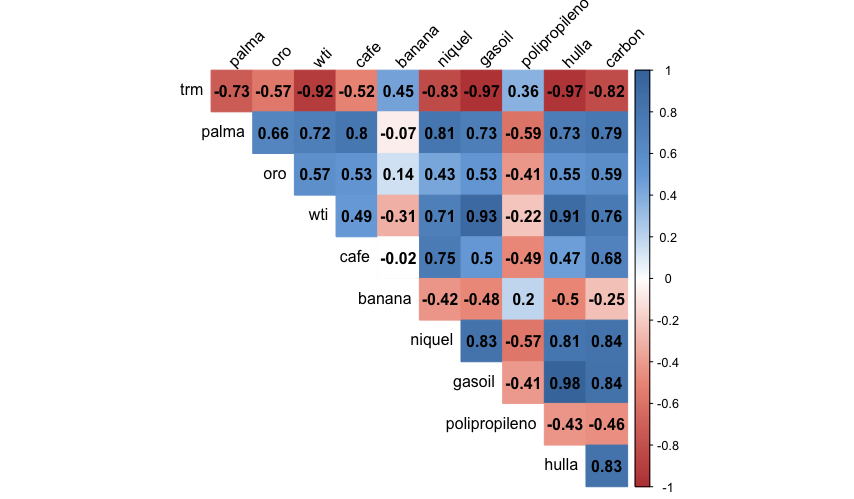
\includegraphics[width = 6 in]{testRegresionMultivariable.png}
    \caption{Matriz Series de Tiempo 2010-2017 Modelo Regresión Lineal}
\end{figure}

Posterior al análisis EDA se procedió a entrenar los datos con un modelo de regresión lineal multivariable.

\begin{itemize}
  \item Los juegos de datos se dividieron en un 70\% de entrenamiento y un 30\% de test.
  \item Para la creación de juegos de datos de entrenamiento y test aleatorios y balanceados se utilizó las funciones de partición de datos de la biblioteca \emph{CARET} del lenguage R.
  \item La función de entrenamiento utilizó la serie de tiempo TRM como variable dependiente y las diez series de tiempo restante como regresores.
  \item La función utilizada como método de entrenamiento fue \emph{glm} para permitir el uso de métodos generales de regresión con transformación de variables.
\end{itemize}

Los resultados del modelo entrenado con la biblioteca \emph{CARET} fueron los siguientes:

\begin{lstlisting}[language=R]
> summary(modelFit)

Deviance Residuals:
    Min       1Q   Median       3Q      Max
-380.15   -55.05     1.97    49.72   362.59

Coefficients:
                Estimate Std. Error t value Pr(>|t|)
(Intercept)    7.083e+03  1.211e+02  58.500  < 2e-16 ***
palma          2.256e-01  3.227e-02   6.989 3.75e-12 ***
oro           -2.938e-01  1.703e-02 -17.248  < 2e-16 ***
wti            1.022e+00  3.608e-01   2.832  0.00467 **
cafe          -6.847e-01  1.043e-01  -6.567 6.49e-11 ***
banana        -4.348e-01  4.883e-02  -8.905  < 2e-16 ***
niquel        -2.411e-02  1.251e-03 -19.270  < 2e-16 ***
gasoil        -7.391e-01  5.465e-02 -13.525  < 2e-16 ***
polipropileno -2.196e+01  1.023e+00 -21.479  < 2e-16 ***
hulla         -2.074e-01  8.377e-03 -24.761  < 2e-16 ***
carbon         7.783e+00  4.580e-01  16.991  < 2e-16 ***
---
Signif. codes:  0 '***' 0.001 '**' 0.01 '*' 0.05 '.' 0.1 ' ' 1

(Dispersion parameter for gaussian family taken to be 7893.668)

    Null deviance: 569092627  on 2046  degrees of freedom
Residual deviance:  16071508  on 2036  degrees of freedom
AIC: 24192

Number of Fisher Scoring iterations: 2

Generalized Linear Model

2047 samples
  10 predictor

No pre-processing
Resampling: Bootstrapped (25 reps)
Summary of sample sizes: 2047, 2047, 2047, 2047, 2047, 2047, ...
Resampling results:

  RMSE      Rsquared   MAE
  89.05245  0.9713988  68.24491

\end{lstlisting}

El modelo es el resultante de 2,047 muestras aleatorias utilizando los diez regresores indicados con selección de muestras a través del método bootstrap.

\begin{itemize}
  \item Todos los regresores utilizados contienen valores $p$ menores a 0 con la excepción del petroleo (variable wti) cuyo valor $p$ es menor a 0.001
  \item El error cuadrático del modelo es de 89.05 (esto debe entenderse como 89.05 pesos colombianos).
  \item El coeficiente de determinación del modelo es de $R^2 = 0.97$.
  \item El coeficiente de Criterio de Información de Aikake es de 24192.
\end{itemize}

Podemos reexpresar el siguiente modelo con la fórmula:

\begin{eqnarray*}
    trm_i & = & 7.083e+03 + palma_i(2.256e-01) + \\
& & oro_i(-2.938e-01) + wti(1.022e+00) + cafe(-6.847e-01) +  \\
& & banana(-4.348e-01) + niquel(-2.411e-02) + \\
& & gasoil(-7.391e-01) + polipropileno(-2.196e+01) + \\
& & hulla(-2.074e-01) + carbon(7.783e+00) + \epsilon \\
\end{eqnarray*}

\subsection{Validación del Modelo Entrenado}
Para la validación del modelo entrenado se procedieron con dos pruebas distintas para verificar el error dentro y fuera de la muestra. Una tercera prueba se aplicó para verificar el error aleatorio y la distribución de los residuales, con la intención de detectar cualquier indicio de heterocedasticidad.

La primera prueba revisó los valores reales de la muestra de entrenamiento versus los valores esperados con el modelo de predicción propuesto.

\begin{figure}[H]
    \centering
    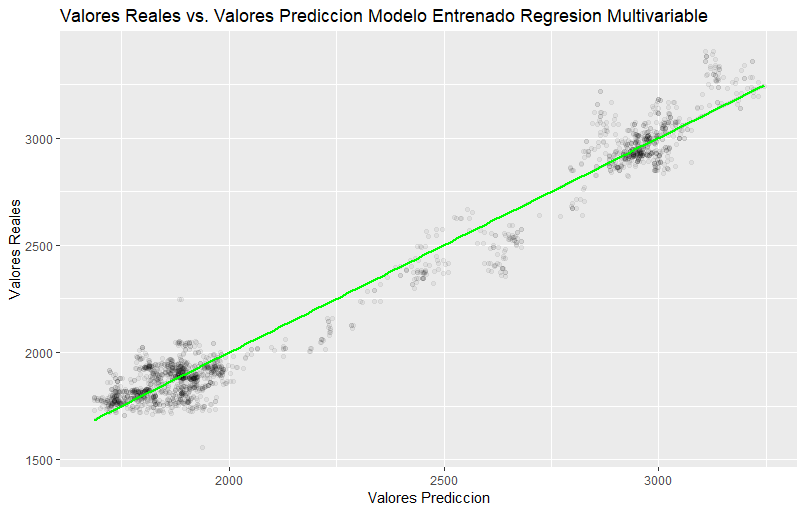
\includegraphics[width = 5 in]{realVStrainingRLM.png}
    \caption{Valores Reales vs. Predicción Modelo Regresión Lineal Multivariable}
\end{figure}

La verificación visual corroboró un ajuste adecuado de los datos con un coeficiente de determinación de 0.9725.

En segundo lugar se procedió a utilizar el modelo entrenado en el juego de datos de evaluación para tener una mejor determinación del posible error fuera de muestra.

\begin{figure}[H]
    \centering
    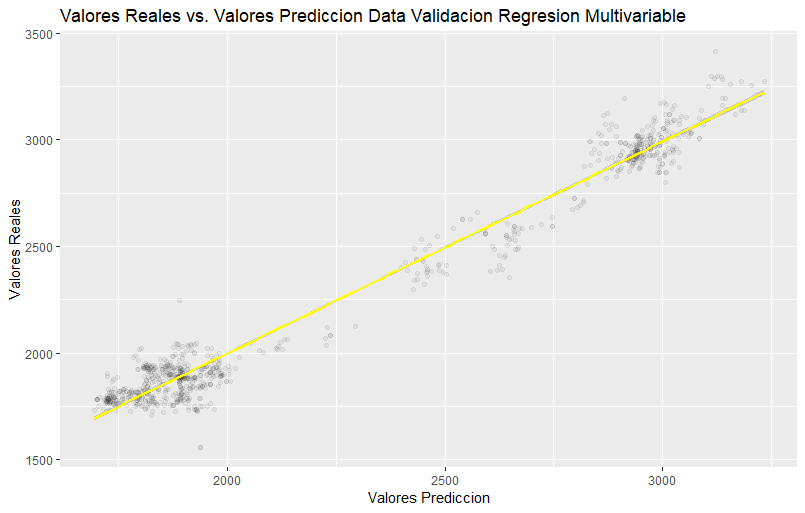
\includegraphics[width = 5 in]{realVStestRLM.png}
    \caption{Valores Reales vs. Predicción Datos de Validación Regresión Lineal Multivariable}
\end{figure}

El modelo se presenta robusto con el juego de datos de validación y el calce de los datos presenta un valor $R^2 = 0.9725$, sin diferencia al modelo de entrenamiento.

En tercer lugar y como última medida, se visualizó la distribución de los residuales para verificar que no había patrón obvio en la distribución de los mismos. La gráfica aplicó una transparencia leve para diferenciar mejor las zonas de mÚltiples puntos de datos. La misma muestra un patrón estacionario similar al ruido blanco que caracteriza la homocedasticidad de los residuales.

\begin{figure}[H]
    \centering
    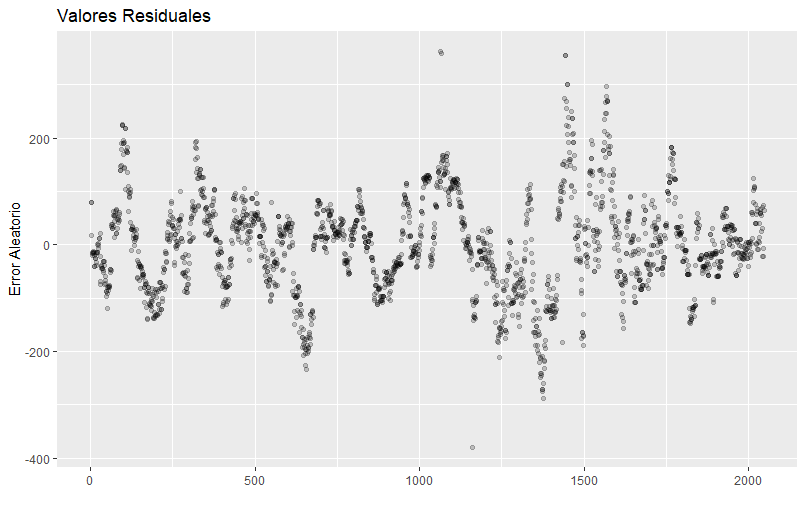
\includegraphics[width = 6 in]{residualesRLM.png}
    \caption{Distribución de Residuales - Validación Regresión Lineal Multivariable}
\end{figure}

\section{Modelo Ensamblado Combinado}
El modelo ensamblado combinado utiliza las predicciones de los dos primeros modelos como entradas para un nuevo juego de datos a entrenar utilizando la misma variable dependiente como variable de predicción y los valores esperados de los dos primeros aprendices como regresores. Es importante notar que los ingresos de los dos aprendices bases no son los valores esperados del modelo de entrenamiento, sino los valores de predicción de ambos aprendices con el juego de datos de evaluación. Esto es importante para reducir el error fuera de muestra en el modelo ensamblado \cite{leek}.

\subsection{Validación de los Datos de Entrada}
Los juegos de datos para los valores de la TRM, los valores esperados del modelo ARIMA, y los valores esperados del modelo de regresión multivariable fueron revisados en una tabla de valores para corroborar que no existan valores extremos o nulos.

\begin{lstlisting}[language=R]
> summary(df_ensamblado)
      trm         predARIMA       predGLM
 Min.   :1557   Min.   :1602   Min.   :1686
 1st Qu.:1828   1st Qu.:1829   1st Qu.:1838
 Median :1933   Median :1932   Median :1928
 Mean   :2259   Mean   :2259   Mean   :2260
 3rd Qu.:2906   3rd Qu.:2908   3rd Qu.:2919
 Max.   :3414   Max.   :3408   Max.   :3245
>
\end{lstlisting}

Como segunda medida, los datos fueron graficados para validar su integridad. El análisis EDA corrobora que no existen valores extremos o nulos.

\begin{figure}[H]
    \centering
    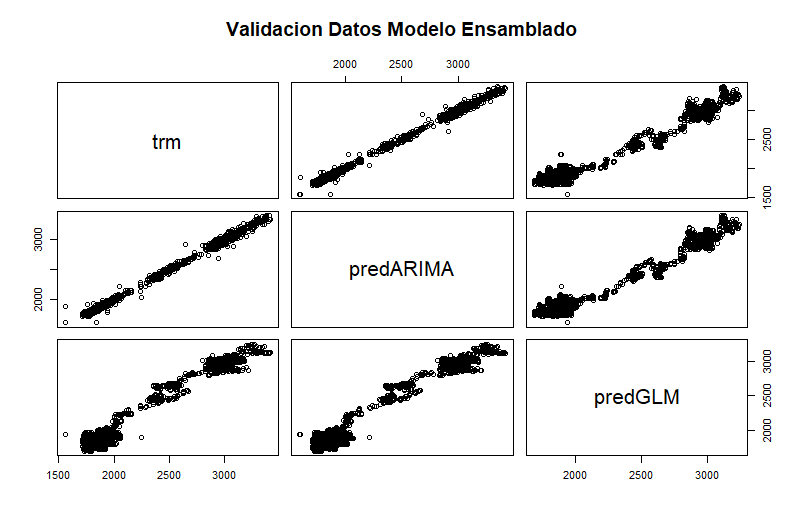
\includegraphics[width = 6 in]{validacionDatosStacking.png}
    \caption{Validación de Datos Modelo Ensamblado}
\end{figure}

\subsection{Entrenamiento de los Datos}
Los datos del modelo ensamblado fueron entrenados utilizando las librerías del paquete \emph{CARET} y con la función GLM (\emph{General Linear Methods}).

\begin{lstlisting}[language=R]
> summary(modeloEnsamblado)
Deviance Residuals:
     Min        1Q    Median        3Q       Max
-103.527    -7.944    -1.092     6.395   224.131

Coefficients:
            Estimate Std. Error t value Pr(>|t|)
(Intercept) 2.462066   3.641217   0.676   0.4991
predARIMA   0.969622   0.009480 102.281   <2e-16 ***
predGLM     0.029860   0.009536   3.131   0.0018 **
---
Signif. codes:  0 '***' 0.001 '**' 0.01 '*' 0.05 '.' 0.1 ' ' 1

(Dispersion parameter for gaussian family taken to be 574.5714)

    Null deviance: 236421477  on 874  degrees of freedom
Residual deviance:    501026  on 872  degrees of freedom
AIC: 8047.6

Number of Fisher Scoring iterations: 2
R-sq.(adj) =  0.998
>
\end{lstlisting}

Las características del modelo final ensamblado fueron las siguientes:

\begin{itemize}
  \item La librería CARET utilizó la familia de funciones de regresión como función aprendiz
  \item Los regresores de la función ensamblada tienen ambos valores p muy bajos: $p = 0.0018$ para el regresor representado por los valores esperados del aprendiz de regresión multivariable, y $p = 2e-16$ para el regresor representado por los valores esperados del aprendiz ARIMA.
  \item El error cuadrático del aprendiz ensamblado es 24.02.
  \item El valor del coeficiente de determinación del modelo ensamblado es $R^2 = 0.998$
\end{itemize}

De esta forma podemos formalizar la ecuación del modelo ensamblado final de la siguiente manera.

\begin{equation}
    p^{c}(trm_i) = (p^{c}(c_{1} \mid trm_i),p^{c}(c_{2} \mid trm_i))
\end{equation}

Donde:

\begin{equation}
    c_{1} : \Delta trm_t = -0.3578 \Delta trm_{t-1} + 0.2932 \Delta trm_{t-2} - 0.1187 \Delta trm_{t-3} + 0.2176 \epsilon_{t-1} - 0.4763 \epsilon_{t-2}
\end{equation}

donde $\Delta = trm_{t} - trm_{t-1}$ y

\begin{eqnarray*}
    c_2 : trm_i & = & 7.083e+03 + palma_i(2.256e-01) + \\
& & oro_i(-2.938e-01) + wti(1.022e+00) + cafe(-6.847e-01) +  \\
& & banana(-4.348e-01) + niquel(-2.411e-02) + \\
& & gasoil(-7.391e-01) + polipropileno(-2.196e+01) + \\
& & hulla(-2.074e-01) + carbon(7.783e+00) + \epsilon \\
\end{eqnarray*}

La ecuación se reduce al modelo ensamblado como:

\begin{equation}
    trm_i = 2.462066 + c_1(0.969622) + c_2(0.029860) + \epsilon
\end{equation}

\subsection{Validación del Modelo Entrenado}
Para la validación del modelo entrenado se procedió con dos pruebas: una visual de valores pronosticados versus valores visuales y una tabla final comparando el error cuadrático y coeficiente de determinación de cada modelo a forma de comparación.

\begin{figure}[h!]
    \centering
    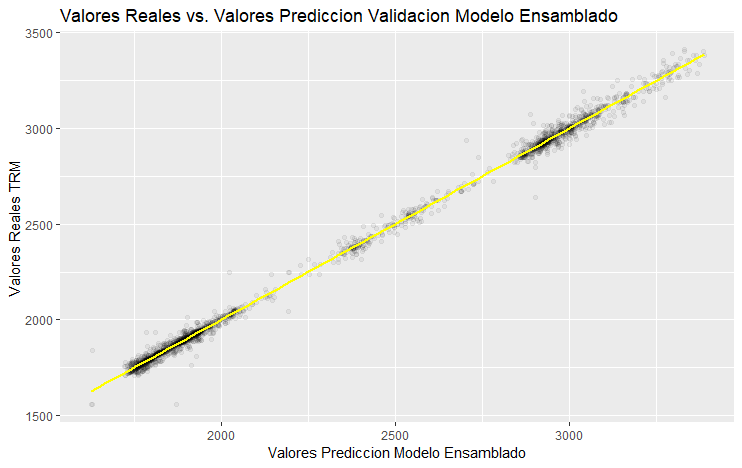
\includegraphics[width = 6 in]{validaCalceStacked.png}
    \caption{Validación Ajuste Modelo Ensamblado}
\end{figure}

La prueba EDA corroboró el ajuste de alta precisión del modelo ensamblado.

Como última medida se construyó una tabla de valores comparativos para verificar el error cuadrático y el coeficiente de determinación de cada modelo.

\begin{table}[h!]
  \begin{center}
    \caption{Desempeño Comparativo de Métodos Machine Learning}
    \label{tab:comparativoMLmetodos}
    \begin{tabular}{c|c|c|c}
      \textbf{Indicador} & \textbf{ARIMA} & \textbf{Regresión Lineal} & \textbf{Modelo Ensamblado}\\
      \hline
      RMSE & 25.5473 &89.0524 & 24.0279 \\
      R2 & 0.9976 & 0.9714 & 0.9978 \\
    \end{tabular}
  \end{center}
\end{table}

La comparación gráfica visual de los tres métodos en un juego aleatorio de prueba se detalla en el cuadro 4.12.

\begin{figure}[h!]
    \centering
    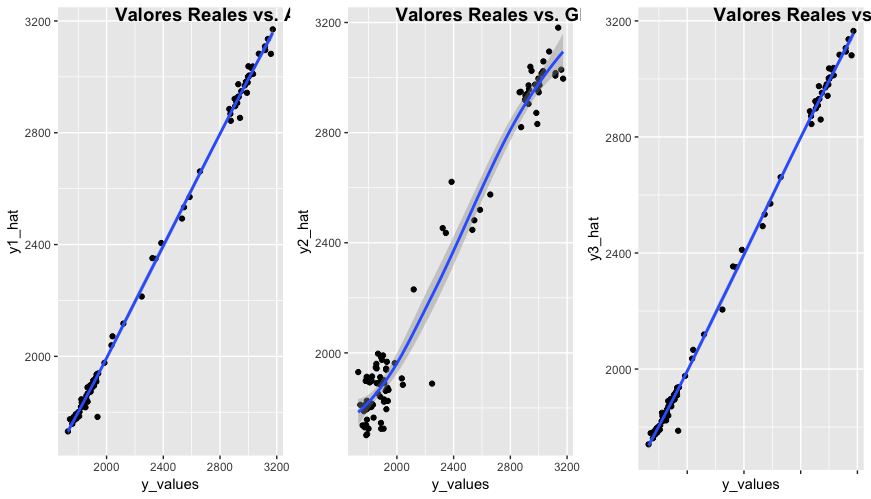
\includegraphics[width = 6 in]{3ModelosComparativo.png}
    \caption{Análisis Comparativo de 3 Modelos de Aprendizaje Automatizado en Juego de Prueba Aleatorio}
\end{figure}
